\documentclass[11pt]{article}
\usepackage[margin=1in]{geometry}
\usepackage[T1]{fontenc}
\usepackage{lmodern,amsmath,amssymb,booktabs,graphicx,xcolor,hyperref}
\usepackage[numbers,sort&compress]{natbib}
\usepackage{tikz}
\usepackage{needspace}
\usetikzlibrary{arrows.meta,positioning}
\hypersetup{colorlinks=true,linkcolor=blue,citecolor=blue,urlcolor=blue}
\setlength{\emergencystretch}{2em}
\newcommand{\pending}[1]{\par\smallskip\Needspace{4\baselineskip}\noindent\textcolor{red!65!black}{\textbf{Draft completion item:} #1}\par\smallskip}
\newcommand{\kj}{\ensuremath{\mathrm{kJ\,mol^{-1}}}}
\title{Route-Aware Computational Selection of Redox Motifs for Preformed Polymers}
\author{Working draft: authorship and affiliations to be confirmed}
\date{Evidence snapshot: 22 October 2026}
\begin{document}
\maketitle
\begin{center}\small\textbf{Internal working draft.} Pending calculations and validation are identified explicitly.\end{center}

\begin{abstract}
Selecting redox motifs for an already formed polymer requires a molecular redox screen to be linked to an exact attachment route and a local graft environment. We develop an identity-linked workflow that separates these assessments and preserves their chemical definitions, physical checks and reconstructable evidence. A retrospective MeCN benchmark gives an unfitted mean absolute error of 0.247 V over 39 potentials, while base-assisted grafting calculations expose a shared proton-transfer contribution whose external validation materially limits thermodynamic interpretation. Matched finite-polymer cycles demonstrate how to formulate conditional grafting without assuming a loading distribution; exact end-to-end candidate decisions and converged conformer ensembles remain required before submission.
\end{abstract}

\begin{figure}[htbp]
\centering
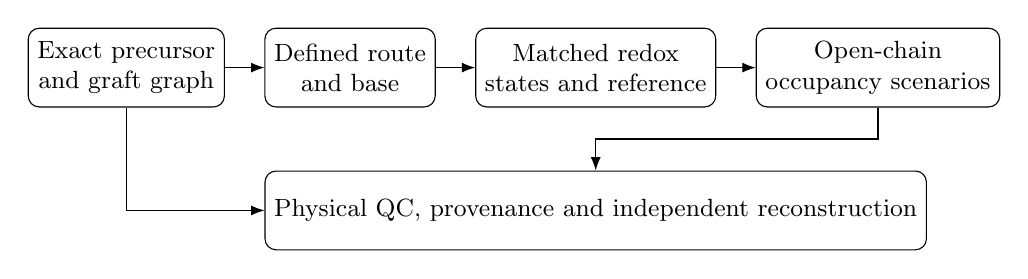
\begin{tikzpicture}[node distance=5mm, every node/.style={draw,rounded corners,align=center,font=\small,minimum height=10mm},>=Latex]
\node (identity) {Exact precursor\\and graft graph};
\node[right=of identity] (route) {Defined route\\and base};
\node[right=of route] (redox) {Matched redox\\states and reference};
\node[right=of redox] (polymer) {Open-chain\\occupancy scenarios};
\node[below=8mm of redox] (qc) {Physical QC, provenance and independent reconstruction};
\draw[->] (identity)--(route);\draw[->] (route)--(redox);\draw[->] (redox)--(polymer);
\draw[->] (identity.south) |- (qc.west);
\draw[->] (polymer.south) -- ++(0,-4mm) -| (qc.north);
\end{tikzpicture}
\caption{Workflow overview. Molecular redox properties, route-dependent grafting thermodynamics and neighboring-site effects are separate outputs linked by exact chemical identity. Execution correctness is evaluated independently of experimental accuracy. The diagram describes the framework and does not imply that every calculation or validation component is complete.}
\label{fig:workflow}
\end{figure}

\section{Introduction}
Redox-active polymers and colloids provide charge-storage architectures that can reduce transport of active groups through separators. Aqueous polymer flow batteries and nonaqueous redox-active colloids establish distinct realizations of that approach.\cite{janoschka2015,montoto2016} Kim and co-workers further demonstrated redox-matched insoluble polymer beads coupled to soluble mediators.\cite{kim2022} For an already formed support, selecting a redox group requires both a useful electrochemical response and a feasible reaction at an accessible polymer site.

High-throughput calculations have explored quinone redox couples and databases have organized redox-active chemical space.\cite{er2015,d3tales2023} Such efforts motivate systematic design, while computational electrochemistry identifies reference, solvation and charge-state errors that complicate transferring potentials between chemical environments.\cite{marenich2014,fc2010,elhajj2024} A potential of a free parent molecule cannot alone establish the behavior of an exact graft. Attachment introduces precursor access, selectivity and reaction conditions; neighboring grafts introduce additional conformational and electrostatic response. Reactive-handle density, conversion, sequence spacing and spatial contact must therefore remain distinct.

General workflow systems already support provenance, failure handling and large quantum datasets.\cite{aiida2020,fireworks2015} The present contribution is their application to chemically explicit, separate decision dimensions: molecular redox response, base-defined attachment and conditional neighboring-site effects (Figure~\ref{fig:workflow}). Exact identities allow evidence to be joined without treating a descriptor, a favorable reaction sum or a stacked geometry as interchangeable proof of feasibility. This working revision reports the validated components and limits its finite-polymer results to method demonstrations pending adequate sampling.

\section{Methods}
\subsection{Molecular identity, candidate generation and attachment routes}
The current synthesis model is post-functionalization of a preformed polymer bearing reactive benzyl chloride sites. A 4-methylbenzyl chloride fragment provides a local capped-site reference. Its grafted products are molecular models of a polymer attachment site; they do not contain the full support, crosslinks or an experimentally measured graft distribution. Earlier vinyl-monomer explorations are kept as a separate historical branch and are not the principal route-selection model.

Systematic designs vary declared viologen, pyromellitic-diimide and naphthalene-diimide cores, attachment linkers, terminal substituents and individual ring substitutions. Exact stereochemical graphs and precursor/product pairs are deduplicated, while every generating recipe is retained. Charge states and multiplicity hints are checked for electron-count consistency. A declared redox ladder remains a computational hypothesis until its states pass the appropriate property-specific checks. Molecular weight and nominal gravimetric capacity, $Q=nF/(3.6M)$, are bookkeeping descriptors; they do not establish accessible electron count, polymer capacity or synthetic feasibility.

The successor route stage reconstructs a charge- and atom-balanced precursor/product pair and a uniquely mapped new heavy-atom bond from each verified upstream design. Evidence is bound to that exact identity, so a precedent for a different product cannot authorize the design. A prospective route gate requires documented precursor access, attachment selectivity, defined reaction conditions, a balanced route, redox-core retention and source evidence. It distinguishes proceed, hold and exclusion decisions. Family-level precedents are retained with their scope and are not automatically promoted to exact-candidate synthesis evidence. Historical calculated properties and explicitly scoped method controls remain available even when a prospective synthesis decision is unresolved.

\subsection{Electronic structure and solution free energies}
Geometry-level and native-Hessian calculations use r$^2$SCAN with D4 dispersion and SMD acetonitrile \cite{r2scan2020,d42019,smd2009}. The geometry-level basis is def2-SVP for neutral and cationic states and def2-SVPD for anions. Active electronic energies use $\omega$B97M-V/def2-TZVPD on the selected geometry, with the same solvent model.\cite{wb97mv2016,def22005,diffuse2010} PySCF 2.14.0 and GPU4PySCF 1.8.1 are the validated implementations for the present native-thermal protocol.\cite{pyscf2020,gpu4pyscf2024} Supporting electrolyte ions are not implicitly introduced into these bare-solute calculations. Explicit ion-pair models are identified separately.

The reported molecular free-energy model is
\begin{equation}
G = E_{\mathrm{SMD}}^{\omega\mathrm{B97M-V}} + G_{\mathrm{nuclear}}^{\mathrm{qRRHO}} - RT\ln(2S+1).
\end{equation}
The nuclear partition uses the solution geometry-level DFT Hessian. Rigid translations and rotations are excluded by a mass-weighted geometric projection, rather than by deleting all frequencies below a numerical threshold. The xTB 6.7.1 thermodynamic kernel is used only as a qRRHO integrator for the explicit DFT internal-mode list.\cite{grimme2012,xtbprogram2021} Frequencies are unscaled. Modes between $-5$ and 0 cm$^{-1}$ are accepted only within the stated minimum tolerance and enter the partition as $|\nu|$; more negative modes fail. The rotational symmetry number is determined by xTB from the exact geometry. The primary rotor cutoff is 50 cm$^{-1}$. Cutoffs of 25 and 100 cm$^{-1}$ provide sensitivity estimates. This use of the thermodynamic kernel does not substitute a semiempirical Hessian for a DFT Hessian. The spin factor assumes an unsplit ground multiplet; unresolved state ordering remains a separate admission issue.

Thermodynamic acceptance requires the largest absolute Cartesian gradient component no larger than $4.5\times10^{-4}$ hartree bohr$^{-1}$, Hessian asymmetry no larger than $10^{-6}$ in the stored atomic-unit matrix, and a lowest internal frequency no smaller than $-5$ cm$^{-1}$. The complete Hessian columns for atom 0/y and the first oxygen/z coordinate are tested at 0.0005 and 0.001 bohr; iron or the final atom is used when oxygen is absent. Each sampled column must meet a 1\% relative-norm error threshold. This tests two columns, not the full Hessian. The absolute spin-contamination threshold is $|\langle S^2\rangle-S(S+1)|\leq0.1$. Full integration-grid response, finite numerical values and spin diagnostics are checked separately. SCF convergence alone is insufficient for thermodynamic admission. Missing thermal or electronic quantities remain missing. Geometry optimization uses geomeTRIC.\cite{geometric2016} The charge-dependent geometry/Hessian basis is a protocol imbalance; a neutral-SVPD sensitivity panel is required before judging its effect, and no basis-convergence claim is made here.

\subsection{Redox reference and retrospective accuracy assessment}
For a one-electron oxidized/reduced pair, potentials are calculated from $G_{\mathrm{ox}}-G_{\mathrm{red}}$ and referenced to a matched ferrocene/ferrocenium calculation. The experimental comparison uses exact free-parent identities and documented acetonitrile measurements with direct or source-defined reference conversion. Lower-tier measurements and excluded events are retained in the source catalog.

The frozen retrospective panel contains 39 potential endpoints from 30 molecules. It includes all currently sourced strict endpoints and is not a held-out test set. Independent reviewers reconstruct state free energies, the reference and potential differences from backing records. Statistics use unrounded calculated potentials, retaining family, redox-step and original-study labels. Molecule- and study-cluster bootstrap summaries use 2,000 replicates and seed 20261021; intervals require at least five clusters. These summaries describe this panel and are not calibrated prediction intervals for new structures. The primary statistics use no fitted offset or outlier removal. Post hoc endpoint-, molecule- and study-held-out offsets are reported separately, using either a single training-set mean residual or separate means for the two redox steps. All endpoints of a held-out molecule or study are excluded together. Because the residual structure motivated these analyses, they are internal diagnostics rather than prospective validation.

\subsection{Defined grafting reactions and standard states}
For an N--H or O--H precursor, the local reference reaction is
\begin{equation}
\mathrm{RCl + HNu \rightarrow RNu + HCl}.
\end{equation}
Pyridyl quaternization is treated as a distinct reaction class with the appropriate precursor and chloride charge. The neutral-substitution reference is not interpreted as the actual free energy of a synthesis that includes a base. For a defined base $\mathrm{B}$, we additionally evaluate
\begin{align}
\mathrm{RCl + HNu + B} &\mathrm{\rightarrow RNu + BH^+ + Cl^-},\\
\mathrm{RCl + HNu + B} &\mathrm{\rightarrow RNu + [BH^+\cdots Cl^-]}.
\end{align}
The separated-ion and contact-pair representations are alternative thermodynamic models, rather than an assumed equilibrium population or a precipitation model. Each reaction is checked for atom and charge balance.

The native thermal translation convention is ideal-gas 1 atm. Reaction sums are converted to a 1 M solute standard state by adding $\Delta nRT\ln(RTc^\circ/p^\circ)$. The correction cancels for the neutral reference and separated-ion routes and is approximately $-7.93$ \kj\ for the contact-pair route at 298.15 K. The DBU/DIPEA pilot computes each neutral base, protonated base and protonated-base/chloride contact pair. Three geometry seeds are evaluated per new species, and thermochemistry is applied to the selected electronic-energy minimum. Reused component values retain their original source hashes. The difference between paired and separated representations is a model sensitivity, not an uncertainty interval.

A separate external term check compares $\mathrm{B+HCl\rightarrow BH^++Cl^-}$ with the author-maintained MeCN basicity collection and recommended acid table.\cite{basicity2019,acidity2013,pkaTables} The conversion is $\Delta G^\circ=-RT\ln(10)[\mathrm{p}K_a(\mathrm{BH^+})-\mathrm{p}K_a(\mathrm{HCl})]$. Base identity is matched by the exact neutral molecular graph; analogues are not substituted. This comparison uses 298.15 K, while exact source temperature and activity conventions remain under review. HCl cancels from the full all-DFT grafting cycle. Replacing only its capture term therefore tests sensitivity to a term and shared-error cancellation; it does not calibrate the complete reaction.

\subsection{Finite-polymer construction and conditional occupancy cycles}
Oligomer construction preserves an open carbon backbone, the intended graft bond and declared stereochemistry. Monomers, dimers and trimers are included in the original interaction panel; no tetramers are included. GFN2-xTB/ALPB(acetonitrile) warm starts provide conformational seeds for subsequent DFT evaluation.\cite{gfn22019,alpb2021} Starting pose labels do not determine the final contact class. XYZ audits independently inspect composition, bonding, stereochemistry and severe clashes.

The matched spacing control uses a five-repeat backbone with reactive sites 2, 3 and 4 and plain styrene end-padding units at positions 1 and 5. The six occupancy graphs are empty, singly grafted at sites 2, 3 or 4, and doubly grafted at 2/3 or 2/4. Unreacted benzyl chloride and unfunctionalized styrene units remain chemically distinct. The graft is a neutral phthalimide method control. The initial search uses seed 20261020, four embedded structures and two xTB seeds per starting mode, with two selected DFT poses per graph giving twelve electronic calculations. Unbiased starts are supplemented by open and slipped starts for double grafts. One declared backbone configuration is used; it is not a model of an atactic sequence ensemble. Fully occupied short oligomers represent dense local scenarios; these calculations assign no experimental loading distribution or occupancy probability.

The neighboring-site free-energy nonadditivity is
\begin{equation}
\Delta\Delta G_{ij}=G_{ij}+G_{00}-G_i-G_j.
\label{eq:nonadditivity}
\end{equation}
This quantity is also the difference between grafting the second site in the presence and absence of the first graft when the same reagent and byproduct terms are used. It includes changes in the backbone, conformation and solvent response and is not a pure pendant-core pair interaction. Electronic $\Delta\Delta E$ and thermodynamic $\Delta\Delta G$ are kept separate. An absolute conditional grafting free energy additionally includes the defined base and byproduct terms.

For separate, intact molecular segments, frozen-fragment energies distinguish interaction from deformation:
\begin{align}
E_{\mathrm{int}} &= E_{AB}-E_A^{AB}-E_B^{AB},\\
E_{\mathrm{def}} &= (E_A^{AB}-E_A^0)+(E_B^{AB}-E_B^0).
\end{align}
Their sum equals the segment association energy referenced to relaxed isolated segments. This partition avoids cutting covalent bonds or adding new caps. It nevertheless contains the full segments, is not counterpoise corrected, and does not establish an association free energy or electronic coupling.

\subsection{Evidence and execution controls}
Every reported field points to exact inputs, numerical settings and immutable backing records. Physical checks govern acceptance separately from scheduling success. Durable geometry checkpoints remain unqualified until normal convergence, topology, spin and thermodynamic checks pass. Independent GPU reservations and bounded CPU thread pools govern parallel calculation. Numerical replay, synthetic throughput, CPU concurrency and actual quantum restart controls are reported in the Supporting Information; these test execution or numerical equivalence rather than experimental accuracy.

\section{Results}
\subsection{Systematic designs and benchmark coverage}
The search generates 1,593 recipes corresponding to 837 distinct exact designs in the viologen, PMDI and NDI families. The historical cohort comprises 75 candidates and the same 75 reaction identities, with 72 unique precursors. It is distinct from the 837-design enumeration. No new full-redox campaign was submitted by that enumeration stage; exact graph matches can nevertheless reuse historical calculations with matching state and protocol provenance. The current prospective registry contains family-level sources but no exact-candidate route entries, and all 837 designs remain on hold for synthesis. Two exact historical/enumerated PMDI and NDI matches have been selected for an end-to-end revision; this assessment is not yet complete.

The retrospective free-parent benchmark includes 39/39 sourced potentials from 30 molecules and seven studies, with MAE 0.247 V, RMSE 0.279 V and bias $+0.190$ V (Figure~\ref{fig:benchmark}). Molecule-cluster 95\% bootstrap intervals are [0.213,0.286], [0.245,0.313] and [0.128,0.257] V, respectively. Seven unequal study clusters provide weakly calibrated intervals, reported separately in the SI. An independent reconstruction contains 111 checks with no discrepancies. The final PMDI second-reduction endpoint is included; its alternative triplet lies 0.707 eV above the selected singlet electronically, while the alternative thermal spin gap remains unresolved.

Coverage differs materially from the design space. Twenty-two endpoints are quinones, which are absent from the systematic enumeration. The imide subset contains nine endpoints from six molecules in one study, including three PMDI derivatives and three phthalimides; viologen contributes one molecule, and there is no NDI endpoint. These results define accuracy for the measured free parents and do not validate 837 grafted designs or polymer environments.
\begin{figure}[htbp]\centering
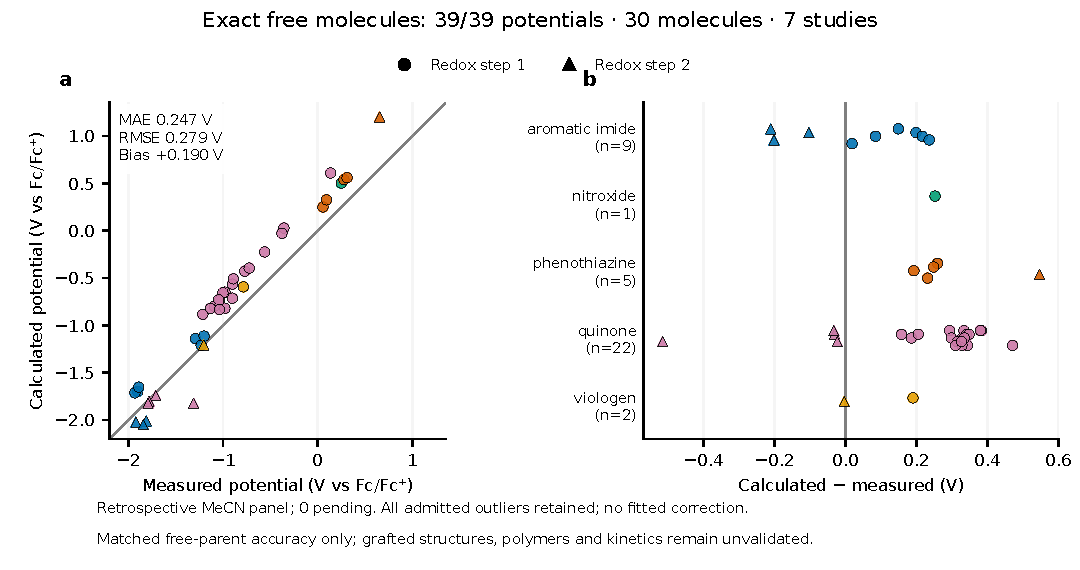
\includegraphics[width=\linewidth]{../results/figures/manuscript/2026-10-22_review_revision/benchmark.pdf}
\caption{Unfitted retrospective benchmark for 39 exact free-parent potentials in MeCN. Family and redox-step labels expose unequal coverage. All sourced endpoints and outliers are retained; no fitted offset is applied.}
\label{fig:benchmark}\end{figure}
\subsection{Reference bias and charge-state errors are distinguishable}
All 30 first-step errors are positive, with mean $+0.266$ V. The nine second-step errors have mean $-0.064$ V and MAE 0.185 V. Their lower MAE can reflect cancellation between systematic contributions and should not be read as superior second-reduction accuracy. Squared bias accounts for approximately 46\% of the overall mean-squared error. A molecule-held-out constant offset reduces MAE/RMSE to 0.158/0.211 V; separate first- and second-step offsets give 0.106/0.166 V. Study-held-out values are 0.182/0.232 and 0.124/0.177 V, respectively (SI). These internal analyses diagnose structure in the residuals while leaving the primary predictions unchanged.

The computed Fc absolute potential is 4.379 V. Stored comparison values, 4.618--4.662 V, use other functionals and cannot be adopted as level-matched replacements. Their difference from the present reference is similar to the positive first-step bias, making a reference contribution plausible. Multiple organic-reference differences that cancel Fc are examined in the SI. Nevertheless, all nine paired step spacings are too large in magnitude: a common reference shift cancels from a spacing and cannot explain this result. Reference, charge-state solvation and ion-pairing errors can coexist. A large quinone study found distinct first/second-reduction intercepts under other methods in DMF versus SCE; it provides relevant precedent, not a numerical calibration for MeCN/Fc.\cite{elhajj2024} A spin-only partition also omits ferrocenium orbital/vibronic contributions; their sign and limiting size are discussed in the SI.\cite{fcorbital2017}
\begin{figure}[htbp]\centering
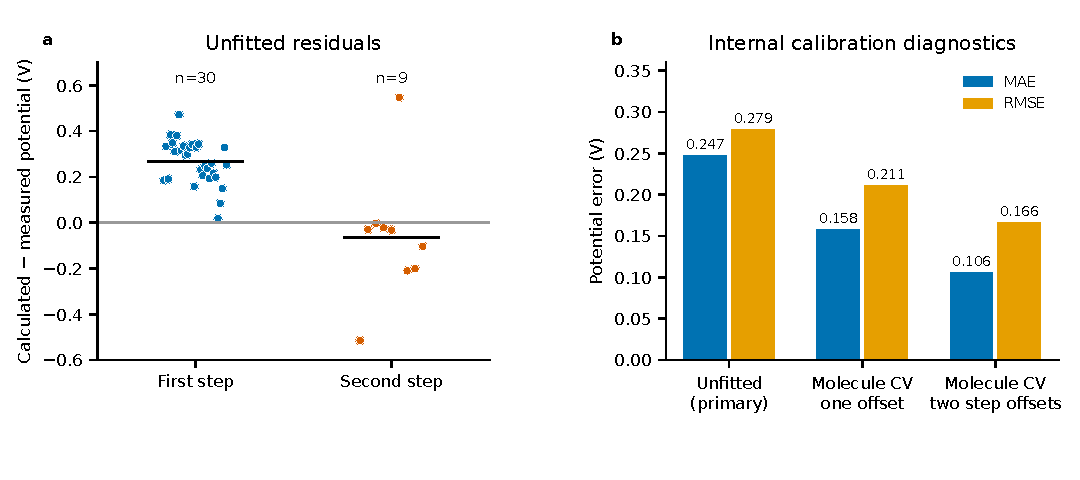
\includegraphics[width=\linewidth]{../results/figures/manuscript/2026-10-22_review_revision/reference_bias.pdf}
\caption{Unfitted step-dependent residuals and internal molecule-held-out offset diagnostics. Training offsets exclude the entire target molecule. Diagnostic calibration is shown separately from the primary benchmark and is not an external test on new compounds.}
\label{fig:reference}\end{figure}
\subsection{A fixed base shifts grafting thermodynamics without changing ranking}
Of 75 local reference reactions, 67 have complete free energies and eight remain held. The base pilot combines five complete candidate reactions with six checked DBU/DIPEA components to give twenty base-assisted values. For a fixed base and ion representation,
\begin{equation}
\Delta G_{\mathrm{graft,B}}=\Delta G_{\mathrm{graft,HCl}}+
\Delta G(\mathrm{B+HCl\rightarrow BH^++Cl^-}),
\end{equation}
with the paired analogue and its standard-state correction defined separately. The separated-ion constants are $-102.78$ \kj\ for DBU and $-70.98$ \kj\ for DIPEA. Thus the base choice can change signs but cannot reorder candidates within a given representation.

The two benzoquinone HCl-reference values, $+57.63$ and $+56.03$ \kj, become $-45.14/-46.75$ \kj\ with DBU and $-13.34/-14.94$ \kj\ with DIPEA. AQ-1-oxy and NDI also change sign in this panel (Figure~\ref{fig:grafting}); this is not a benzoquinone-specific rescue. These values motivate testing a defined base-assisted route, while selectivity, precursor access, salt speciation and support accessibility remain separate route gates.
\begin{figure}[htbp]\centering
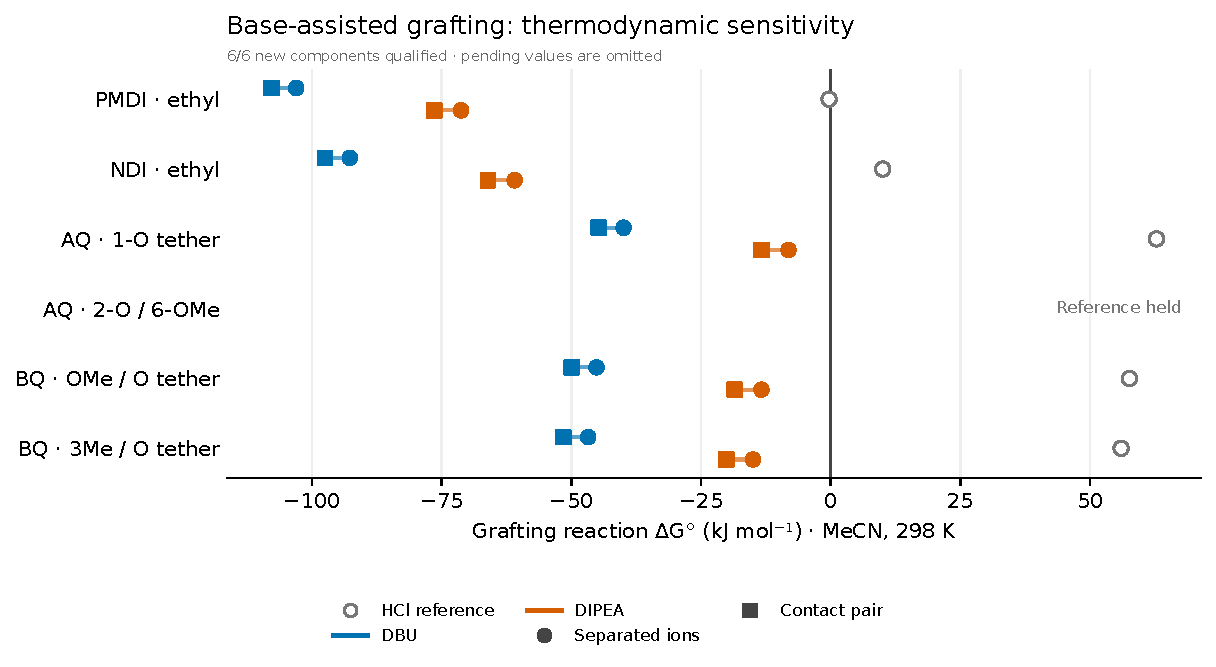
\includegraphics[width=\linewidth]{../results/figures/manuscript/2026-10-22_review_revision/grafting.pdf}
\caption{Candidate HCl-reference reactions plus a constant per-base proton-capture term. Separated ions and contact pairs are alternative thermodynamic representations; their differences do not establish measured ion-pair populations.}
\label{fig:grafting}\end{figure}

The revised MeCN collection gives pKaH(DBU)=24.31 and the recommended acid table gives pKa(HCl)=10.30.\cite{basicity2019,acidity2013,pkaTables} At 298.15 K these imply $-79.97$ \kj\ for capture, versus $-102.78$ \kj\ computed, a discrepancy of $-22.81$ \kj. Replacing only this term leaves the two DBU/BQ sums negative ($-22.33/-23.94$ \kj), but changes shared-error cancellation because HCl cancels from the full DFT cycle. These hybrid sums are sensitivities, not calibrated grafting predictions. Two additional HCl/Cl-free relative-basicity reactions, for pyridine and triethylamine against DBU, differ from the tabulated scale by $+4.58$ and $+1.40$ \kj\ (SI). This narrows the diagnostic without uniquely assigning the capture discrepancy to chloride or HCl. Exact source temperature/activity conventions remain under review. An exact DIPEA MeCN anchor is unavailable in the checked collection; its favorable sign remains conditional, and the DBU discrepancy is not transferred as a DIPEA correction.

\subsection{Conditional grafting is demonstrated in a finite control}
A five-repeat phthalimide model distinguishes reactive sites, plain-styrene end padding and occupied sites. All twelve selected electronic poses and six selected-geometry free energies pass their specified checks. The adjacent and one-spacer cycles give $\Delta\Delta G=-5.15$ and $-11.23$ \kj. These include conformational, backbone and solvent response and do not measure a pure motif pair interaction. The exact occupancy model, conditional reactions, fragment decomposition and numerical checks are presented in the SI.

The initial two-DFT-pose sampling and single backbone configuration do not support a spacing design rule or an equilibrium ensemble. Rotor-cutoff sensitivity, below about 1 \kj\ for these cycles, does not bound conformer uncertainty. These results therefore remain a methods demonstration. Broader conformer searches, multiple backbone configurations, DFT re-ranking and a defined ensemble free energy are required before interpreting a polymer-design trend.

\section{Discussion}
The immediate chemical lesson is to distinguish a molecular descriptor from a route-dependent decision. Base capture contributes a common term rather than a candidate-specific ranking advantage; its external check limits the interpretation of a favorable grafting sum. Likewise, conditional occupancy cycles state what can be computed when graft conversion and spacing are unknown, without inventing a loading distribution. Strong unwanted association is a design concern, but neither neutral nonadditivity nor a stacked geometry establishes an electron-transfer rate or full-bead transport behavior.

The benchmark identifies a sizeable common bias and a separate step-dependent component. Reference cancellation, grouped cross-validation and paired spacings offer complementary diagnostics; none alone attributes error uniquely to Fc. Changing the fitted offset or charge-state protocol now would require a declared calibration set and a separate external test before claiming improved predictive accuracy.

The principal limitations are incomplete end-to-end examples, uncertain exact synthesis routes, restricted benchmark coverage, the charge-dependent geometry/Hessian basis, incomplete conformer sampling and continuum-ion/speciation uncertainty. The pipeline preserves those distinctions, but bookkeeping cannot substitute for the missing chemical evidence. Public raw-state packaging, portable deployment and an archival release also remain necessary. Implementation tests in the SI support traceability and recovery within their stated controls and do not establish million-molecule quantum throughput.

\section{Conclusions}
An identity-linked workflow can keep molecular electrochemistry, defined attachment reactions and conditional polymer environments comparable while retaining separate evidence requirements. The present results quantify retrospective redox errors, expose a constant and externally testable base contribution, and demonstrate matched occupancy cycles in a finite control. End-to-end exact-candidate assessment, conformer and basis sensitivity, and a portable archival release remain submission requirements for this working revision.

\section*{Supporting Information}
Benchmark intervals and grouped offset diagnostics; relative-basicity controls; finite-polymer construction and conditional cycles; electronic fragment decomposition; numerical implementation, concurrency and quantum restart controls; evidence terminology.
\section*{Data and code availability}
The immutable evidence epoch and source hashes are recorded under \path{manuscript/evidence/2026-10-22_review_revision/}. Versioned code and curated metadata are maintained in the project repository. Bulk calculation records remain on shared storage with recorded identities and hashes. A public archive containing accessible state records, a locked environment and cached-record reproduction examples remains to be completed before submission.
\section*{Author contributions, funding and competing interests}
These statements require confirmation by the authors and are intentionally not inferred in this working draft.
\bibliographystyle{unsrtnat}\bibliography{references}
\end{document}
